\documentclass[a4paper,12pt]{article}
\usepackage[utf8]{inputenc}
\usepackage{graphicx}
\usepackage{caption}
\usepackage{listings}
\usepackage{color}


\definecolor{lightgray}{gray}{0.5}


\lstset{ %
language=Python, 
basicstyle=\ttfamily,
numbers=left,               
numberstyle=\footnotesize, 
numbersep=5pt, 
showspaces=false, 
showstringspaces=false,
showtabs=false,
commentstyle=\color{lightgray},
frame=false,
tabsize=2,	              
captionpos=t,            
breaklines=true,              
breakatwhitespace=false,      
title=\bf\lstname,                 
}

\newcommand{\ditem}[1]{\item[\texttt{{#1}}] \hfill \\}

\begin{document}
\title{Flexible Presenter Tools for e-Learning}
\author{Student: Christian Panton\\
Supervisor: Henrik Madsen}
\date{October 4th, 2010}

\maketitle
\newpage

\tableofcontents
\vspace{20 mm}
All HTTP links retrieved October 4th, 2010.
\newpage


\section{Introduction and Context}
The wealth of knowledge held by educational institutions is often kept secret or hidden from public view. Although most hide it intentionally, for institutions who wants to be open, the tools available to the teachers tends to keep knowledge bound to non-digital or propitiatory formats. Some open alternatives have developed, such as MIT OpenCourseWare, but all the components of a full open ecosystem is hard to come by\footnote{http://primer.grafiki.org/index.php/Related\_projects}. The project tentatively named The Universal Primer Project (TUPP), seeks to create such an ecosystem, partly though tools for teaching and partly though tools for knowledge storage and dependency of knowledge.

This project aims to create one of parts needed in the tools for teaching. Software that can stream live video and broadcast slides of lectures for distance learners is not available as an open source ecosystem (clients and servers), and the teachers client seems to be one of the first places to start. Ideally this would all run in a internet browser, but even the most current revision of the HTML standard, would not enable us to interface with hardware such as pointing devices and cameras and provide the performance needed to stream live video. Although 3rd party plug-in technology might exist, such as Adobe Flash, these are propitiatory formats and requires the user to install software.

\section{Development of the Presenter Tool - \emph{emcee}}
Due to the limited functionality of the current open standards based browser technologies, a stand-alone Python application was developed (See Appendix C for the source code). Its purpose is to support the teacher in presenting slides, setting up the live video and audio feeds and provide communication with the distance learners. The application is named after a Master of Ceremonies, the \emph{Em-Cee}.

Python\footnote{http://www.python.org/} is a dynamically typed, object orientated, interpreted programming language. Thus it is a very high-level language and was chosen for its rapid development features. Among those are its large standard library, excellent documentation and broad usage. 

For the Graphical User Interface, \emph{GUI}, the Qt4\footnote{http://qt.nokia.com/} library was chosen. Like Python it is licensed under the GNU General Public License and freely available and it is implemented on all major platforms, ensuring cross-platform compatibility. Although the application is being developed with a target platform of Ubuntu Linux 10.04, it will lower the effort required to port the application to another platform. The Qt4 C++ library is accessed though the PyQt4\footnote{http://wiki.python.org/moin/PyQt4} bindings. Another set of bindings, \emph{PySide}, is currently being developed Nokia and is largely API compatible with PyQt4, but was disregarded due to the lack of maturity of the project.

The application is incorporating a large number of different API's, hardware and network communication and a lot of glue-code, to keep everything working together. The focus has been on developing the glue-code and using existing libraries when available. While the core Python library is very well documented, a lot of the third party libraries are sparsely documented - often only using code examples.
 
\section{Functionality Overview}

The main screen is depicted in figure \ref{fig:mainwindow}. It shows the teacher the current slide and the upcoming slide, side by side. Additionally a list of all the slides is kept in a sortable list below the upcoming slide. This enables the teacher to sort the slides while giving a presentation. By clicking on a slide this also enables the teacher to set the upcoming slide, ie. to skip a series of slides, go back in the presentation during an Q\&A session, etc. 

\begin{center}
	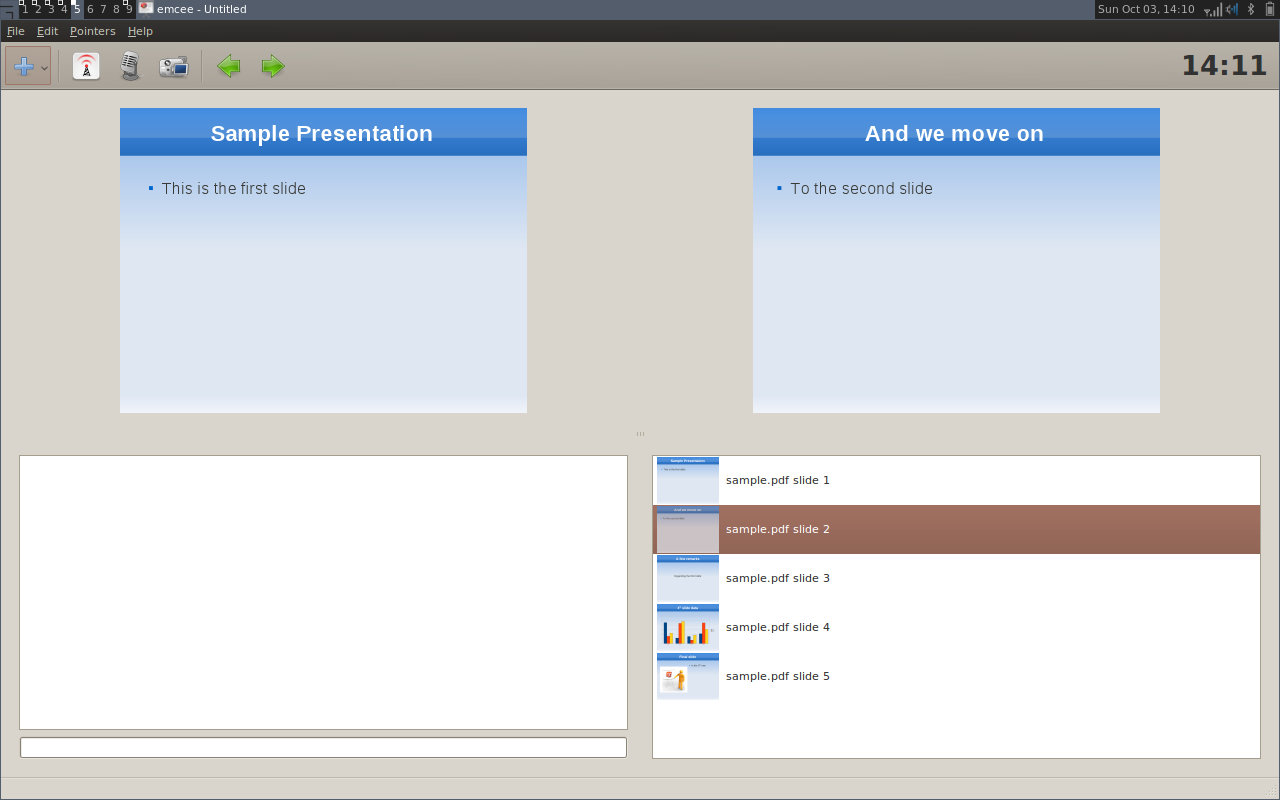
\includegraphics[scale=0.3]{screen.png}
	\captionof{figure}{The main window of emcee. Upper left quadrant: Current slide view (also mirrored on a secondary screen). Upper right quadrant: Upcoming slide. Lower left quadrant: Chat and questions window. Lower right quadrant: Next slide chooser, slide sorter and list.}
	\label{fig:mainwindow}
\end{center}

On the main screen there is also a chat window, which makes it possible for the teacher to write text based messages to the distance learners and makes it possible for the distance learners to ask questions to the teacher. 
A toolbar is also available for adding additional slides, toggling of video, audio and slide broadcasting and to provide information, such as the current time.

The control of the presentation (going forward, etc.) and the types of media available on the slides, is controlled though a simple plug-in system. Python scripts residing in the \texttt{plugins/} folder are automatically loaded into to program. The currently supported plug-in types are pointing devices and slide content. See Appendix \ref{pluginstruct} for the plug-in structure.

\subsection{Pointing Devices}
Pointing devices is a broad category of keyboards, mice and remote controls for controlling the flow of and annotating the presentation. As they are plug-in based, two pointing devices were implemented. 
\\

The first one is a simple keyboard based flow control. It only implements a forward and backwards button, either as the arrow keys or the page-up and down keys. The main reason for also implementing page-up and down keys, is that a large number of wireless remote controls use these keys. It was tested using a cheap no-name 2.4GHz wireless remote control\footnote{http://www.dealextreme.com/details.dx/sku.3071} which enumerates as a USB HID keyboard on the host computer.
\\

The second devices is much more sophisticated. Originally developed for the Nintendo Wii gaming console system, the Wii Remote or \emph{Wiimote} is ideal as a pointing device. The device can be seen in figure \ref{fig:wiimote}.

\begin{center}
	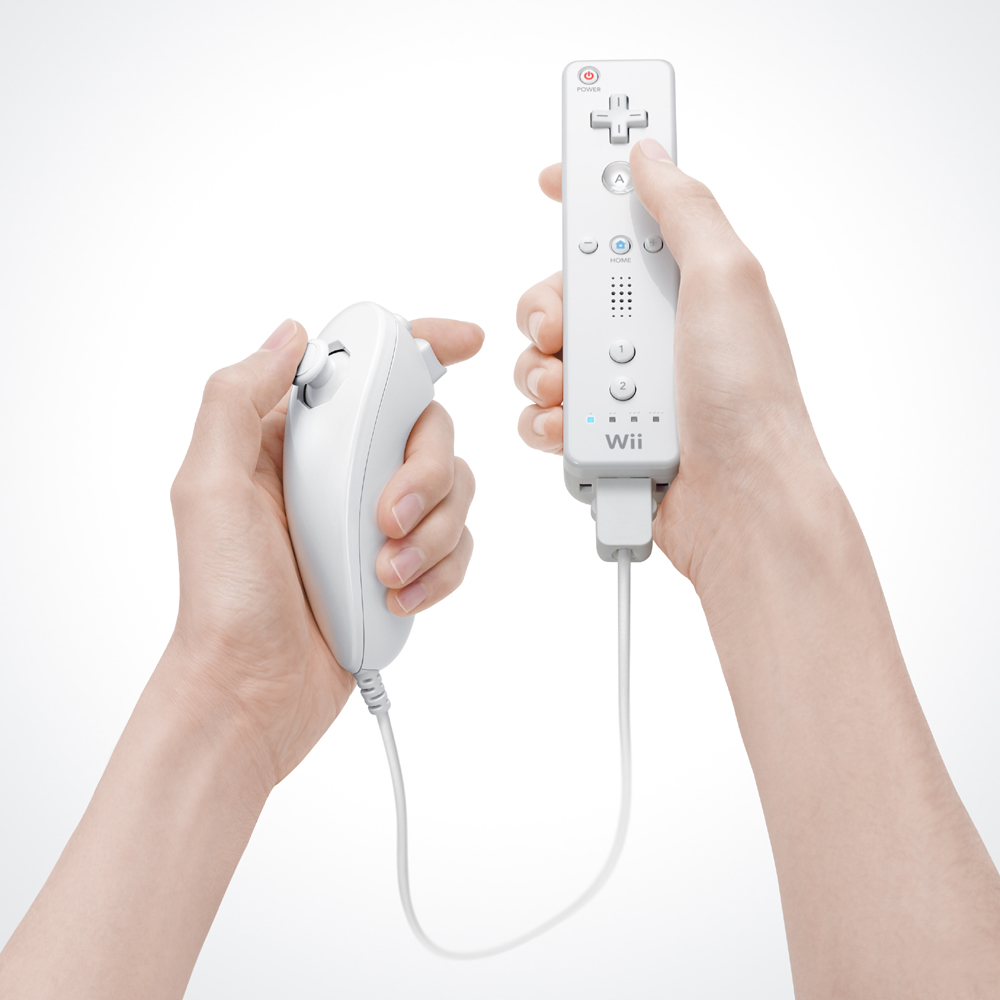
\includegraphics[width=0.70\textwidth]{wiimote.jpg}
	\captionof{figure}{The Wiimote (right) and the Nunchuck (left)}
	\label{fig:wiimote}
\end{center}

The Wiimote is using the wireless Bluetooth communication protocol, which means that it can communicate with most modern laptops. It features a large number of buttons, 3-axis accelerometers, an $I^2C$ communications port (for the Nunchuck, and other peripherals), vibration motor, LEDs and a 4 point-tracking infra-red camera.

A number of Python libraries emerged when developers discovered how the communication protocol worked, but most of them were left abandoned. The CWIID\footnote{http://abstrakraft.org/cwiid/} library was chosen for its maturity, as it is available as a binary package for most Linux distributions. One thing all the libraries have in common is the lack of proper Bluetooth pairing\footnote{http://wiibrew.org/wiki/Wiimote\#Bluetooth\_Communication}. The Wiimote can be placed in two modes. Host (PC) initiated communication and Wiimote initiated communication. Only the host-initiated is implemented, as it is much simpler to use, although it has the downside that the Wiimote has to be put into \emph{discoverable} mode every time you want to connect to it. This is done by pressing the 1 and 2 buttons on the remote simultaneously. Although this is a cumbersome procedure, this skips the step of host-remote pairing and makes sure that Wiimotes can be used interchangeably between computers. 

The Wiimote is used for presentation flow control using the left and right arrow keys. The vibration motor is used to get attention from the teacher, such as getting a question from a distance learner. But the primary reason to use a Wiimote over a much simpler remote, is the infra-red point-tracking camera. By placing two clusters of IR-diodes above or below the projector screen, the Wiimote can be used as a digitized laser pointer. The IR diodes will show up as two points on the IR-camera and its build-in computer vision algorithm sends the positions of the diodes to the host computer. A simple algorithm was written based on the midpoint of the two points and it includes a small correction for rotation of the Wiimote. Pressing a button on the remote enables the teacher to draw on the screen. A vertex reduction algorithm is used to limit the amount of points created by the freehand drawing. 

The Wiimote was intended to be used like this as a mouse. but another configuration is also very popular. Although not implemented in this software, if the Wiimote is placed on a stand, using a pen with an IR-diode in the end, the projector screen can be used as blackboard\footnote{http://johnnylee.net/projects/wii/}. This alternative configuration is worth considering in a future revision of the program, as the accuracy of the drawing is much higher. Using the plug-in system, it is a trivial task to add such functionality.

The digitization of the pointing device is important, as it delivers the same teaching experience to the distance learners as it does to the people in the classroom. The distance learners will be able to see the gestures drawn on the slides by the teacher.

\subsection{Slide Media Support}

In order to support a large amount of different content on the slides, such as PDF files, YouTube videos, etc., the slide content is defined as a plug-in system as well. All content plug-ins are defined by the MIME-type they support. As a matching server-side plug-in is needed, the MIME-type serves as a plug-in identifier.

Implemented in the application is two types of plug-ins. Like with the pointer plug-ins above, a simple and a more advanced plug-in is avaliable.
\\

The simple plug-in is a blank slide. Its MIME-type is the non-standard \texttt{application/x-blank-slide} and can be used to blank the projector between multiple presentation or in a Q\&A session.
\\

The more advanced plug-in is the main content plug-in. It is based on PDF files and has the standard MIME-type \texttt{application/pdf}. Rendering of the PDF files is done by the \texttt{libpoppler} with a set of Python/Qt4 bindings called \texttt{pypoppler-qt4}. 

We had to write a patch for the bindings, as they did not expose the Table of Contents of the PDF file, often used to provide a slide name. The slide name often set by software creating presentations, such as \LaTeX-\texttt{beamer}.

\subsection{Broadcasting Features}

One of the main features of this application is its broadcasting features. They cover slide switching, distance learner chat/question and audio/video broadcast of the lecture.
\\

The audio/video broadcast features has not yet been implemented, as the infrastructure was not available. The foundation for adding this is build into the application and it is implemented as a shell-command.
\\

The slide control (forward, backward, annotation, etc.) and chat protocol named \texttt{CHIMP} has been defined (Appendix \ref{chimpproto}) and implemented in the application.

For each lecture a unique stream-name is given. This acts as an identifier for the media streams, the web page created for the distance learner and in the CHIMP protocol.

The CHIMP protocol is based on the Ajax Push Engine\footnote{http://www.ape-project.org/} (APE) server. APE is made as a JavaScript framework for real-time push of data to websites. It has different methods of communicating, but they rely on standard HTTP requests. A custom Python APE client implementation was written to support this communication. 

The APE client connects to a communication channel, in this case the stream-name. Once in the channel it can send and receive messages from and broadcast to all clients in the channel.
The messages are plain strings and for the CHIMP protocol the strings are URL-escaped JSON\footnote{JavaScript Object Notation, a simple serialization of JavaScript objects, commonly used in web services}. The object created from the unescaped JSON is then used as a remote procedure call in the client. The procedure is determined by the \texttt{type} field. Any other parameters is depended on the procedure, see Appendix \ref{chimpproto} for a listing of different procedures.

\section{Concluding Summary}
As no suiting presenting application was found for the e-Learning project. A custom application was developed.

The application has the basic functionality needed for synchronized slide-casting with chat and annotation features. Video and audio broadcast can be added in a few lines of code once the infrastructure is ready. 

A wealth of different libraries has been used including Wiimote interaction, HTTP asynchronous connection pools (for APE), Qt4 graphic user interface and PDF rending.


%% Appendix
\appendix
\newpage

\section{The CHIMP Protocol}
\label{chimpproto}
The CHIMP Protocol is using APE chat messages as a transport layer. The CHIMP message is URL escaped JSON. Once unescaped, the message type is detected by the \texttt{type} string. From the type, it is possible to determine other fields in the message. The types and fields are described below.

\subsection{CHIMP v1 DRAFT messages}

\begin{description}
\ditem{slides/change}
\texttt{(identifier,index)} Changes the current slide to the slide content identified by \texttt{identifier} (if a file, a md5 checksum of the file) and zero-indexed page identified by \texttt{index}.

\ditem{chat/public-msg}
\texttt{(nickname,msg)} Sends a chat message with content \texttt{msg} and author name \texttt{nickname}.

\ditem{draw/lines}
\texttt{(lines)} Draws lines on the slide. \texttt{lines} is a double array, such that \texttt{[[[$x_0^{line_0}$,$y_0^{line_0}$],[$x_1^{line_0}$,$y_1^{line_0}$],\ldots],[[$x_0^{line_1}$,$y_0^{line_1}$],[$x_1^{line_1}$,$y_1^{line_1}$],\ldots]]]}

\ditem{draw/lines-clear}
Clears any lines drawn on the slide
\end{description}


\section{Plug-in Structure}
\label{pluginstruct}
The plug-in is a Python module. In order to provide a distinction between different plug-in types the string \texttt{plugintype} must be set. Currently supported types are \texttt{pointer} and \texttt{content}.

\subsection{\texttt{pointer}}
In addition to \texttt{plugintype} a few other variables, classes and methods must be defined.

\begin{description}
\ditem{name}
A short descriptive name.

\ditem{description}
A longer description of the plug-in.

\ditem{capabilities}
An array of capabilities of the plug-in. The currently supported are: \texttt{['control','draw','attention','battery']}. Control is flow control, draw is drawing on slides, attention is the capability of notifying the teacher of some event through the device and battery is that the battery can be monitored though an interface provided by the plug-in.

\ditem{enabledefault}
A boolean describing if the plug-in should be loaded at application start.

\ditem{pointer}
A class holding the current pointer.

\ditem{pointer.enable()}
Enable the pointer.

\ditem{pointer.disable()}
Disable the pointer.

\ditem{pointer.battery()}
(Capabilities dependent) Returns the percentage of the battery charge.

\ditem{pointer.xy()}
(Capabilities dependent) Returns a tuple of normalized coordinates (x,y) or None if the pointer is not pointing on the screen.

\ditem{pointer.attention()}
(Capabilities dependent) Try to get some attention.

\end{description}

\subsection{\texttt{content}}
In addition to \texttt{plugintype} a few other variables and methods must be defined.
\begin{description}
\ditem{mimetype}
A string of the MIME-type supported by this plug-in.

\ditem{name}
A short descriptive name.

\ditem{source}
The source type, currently supported: \texttt{file} or \texttt{internal}. If the type is file, a file dialog will be provided by the system for choosing the file.

\ditem{filetype}
(Source dependent) If the source is a file, then this describes the extention of the file, needed for the file dialog.

\ditem{widget(container,index=0)}
Returns a QWidget of the slide in container with index.

\ditem{icon(container,index=0)}
Returns a QIcon of the slide in container with index.

\ditem{container}
A class holding the source for the slides.

\ditem{container(reference)}
Constructor for the container class. Reference is the file path for file-sources.

\ditem{container.numSlides()} 
Returns the number of slides in the container

\ditem{container.getName(index)} 
Returns a descriptive name for the slides at index, ie. from file metadata.

\ditem{container.getIdentifier()} 
Returns a unique identifier for this container. If the container contains the same content, the identifier should be the same across instances. If the source is a file, use a md5 checksum as identifier.

\end{description}

\section{Source code}
Source code is listed below and available at:
\\
\texttt{http://github.com/UniversalPrimer/emcee-gui-client}. 
\\
\\
The revision for this report is \texttt{954beaf775bd3349c1fd}.
\\

\subsection{README}
\lstinputlisting{../emcee-gui-client/README}
\subsection{emcee}
\lstinputlisting{../emcee-gui-client/emcee}
\subsection{ape.py}
\lstinputlisting{../emcee-gui-client/ape.py}
\subsection{controller.py}
\lstinputlisting{../emcee-gui-client/controller.py}
\subsection{gui.py}
\lstinputlisting{../emcee-gui-client/gui.py}
\subsection{plugins.py}
\lstinputlisting{../emcee-gui-client/plugins.py}
\subsection{plugin: blank.py}
\lstinputlisting{../emcee-gui-client/plugins/blank.py}
\subsection{plugin: keyboard.py}
\lstinputlisting{../emcee-gui-client/plugins/keyboard.py}
\subsection{plugin: pdf.py}
\lstinputlisting{../emcee-gui-client/plugins/pdf.py}
\subsection{plugin: wiimote.py}
\lstinputlisting{../emcee-gui-client/plugins/wiimote.py}
\subsection{presentation.py}
\lstinputlisting{../emcee-gui-client/presentation.py}
\subsection{util.py}
\lstinputlisting{../emcee-gui-client/util.py}
\subsection{pypoppler-qt4.patch}
\lstinputlisting{../emcee-gui-client/pypoppler-qt4.patch}




\end{document}
  
